\chapter{Propostas Tecnológicas}

A análise de dados é uma disciplina essencial que desempenha um papel fundamental na tomada de decisões estratégicas e no impulsionamento dos negócios. Com o avanço da era do Big Data, onde uma quantidade massiva de informações é gerada e coletada diariamente, as empresas têm reconhecido cada vez mais a importância de investir em tecnologias e práticas analíticas para extrair insights acionáveis a partir desses dados. Esses insights podem fornecer uma visão abrangente do mercado, identificar oportunidades de crescimento, otimizar operações e melhorar o atendimento ao cliente, conferindo uma vantagem competitiva significativa às organizações que são capazes de aproveitar ao máximo a análise de dados em suas estratégias de negócio \cite{mayer2013big, chen2012business, reddy2013data, watson2010current, white2012hadoop}.

Com essas informações organizadas e disponíveis, tais empresas podem direcionar seus serviços de maneira mais eficaz, desenvolvendo estratégias baseadas em dados concretos e atualizados, contribuindo para o sucesso de seus negócios \cite{chen2012business}.
Entretanto, para transformar esses dados brutos em informações úteis, é necessária uma série de operações, muitas vezes resumidas no processo de Extração, Transformação e Carga (ETL). Este processo envolve a coleta de dados de várias fontes, a transformação desses dados para um formato adequado para análise, e, finalmente, a ingestão dos dados transformados em um sistema de destino para fácil acesso e análise \cite{vassiliadis2002conceptual}.

A adoção de um banco de dados é fundamental para a efetiva implementação do processo de ETL e análise de dados em empresas. Um banco de dados confiável e eficiente desempenha um papel crucial na organização e armazenamento dos dados coletados, permitindo que sejam facilmente acessados e utilizados para análise \cite{elmasri2019fundamentals}. Um banco de dados relacional é uma opção comumente adotada pelas organizações, pois oferece a capacidade de estruturar e relacionar os dados de forma coesa, tornando-os mais compreensíveis e significativos para os usuários \cite{date2003introduction}. Com a utilização de um banco de dados relacional, as empresas podem realizar consultas complexas e obter insights valiosos por meio de operações de junção e agregação dos dados \cite{connolly2014database}. Além disso, a integridade dos dados é assegurada por meio de restrições e relacionamentos definidos no banco de dados, garantindo a consistência dos dados ao longo do tempo \cite{silberschatz2019database}.


A empresa em questão é uma provedora de internet, que atua no mercado B2B (Business to Business), ou seja, atende outras empresas. A empresa possui cerca de 100 funcionários, e está localizada na cidade de São Paulo. Atualmente a empresa utiliza as informações do site da Receita Federal para obter os dados cadastrais dos CNPJs que são abertos no Brasil. Essa informação é utilizada para que o time de prospecção do cliente possa realizar o primeiro contato para oferecer os serviços da empresa. Atualmente, os dados dessa empresa são disponibilizados em um servidor on-premisse, onde um time realiza a extração dos dados do site da receita federal e disponibiliza em um arquivo excel, que é compartilhado com os times de prospecção do cliente e análise de dados através desse servidor. Boa parte desse processo exige a atuação humana, o que torna o processo lento e suscetível a erros. 

As construções dos paineis do time de análise também se baseiam nesses arquivos Excels e quando ocorre a atualização erronea desse arquivo, os painéis tendem a apresentar informações incorretas, ou até mesmo apresentar erro na própria ferramenta. Além disso, a informação não é estruturada da maneira correta, o que dificulta a análise dos dados e a tomada de decisão. Por fim, a informação não é atualizada com tempo hábil para prospecção do cliente, dando uma desvantagem competitiva para a empresa.

Este projeto tem como objetivo construir uma solução que seja em sua maior parte automatizada, realizando os processos atuais de forma 
mais eficiente e com menos intervenção humana. É do interesse também da empresa preservar os custos atuais, ou até mesmo reduzi-los. Considerando esse requisito e o objetivo do projeto, a solução proposta é a adoção de uma solução em nuvem, que permita a escalabilidade e o processamento eficiente dos dados. A solução proposta também envolve a passagem de conhecimento, bem como workshops com os times interessados para a apresentação e treinamento da solução proposta.

Para melhor entender o que a solução deverá realizar, é importante que seja feito uma coleta de requisitos junto ao time de tecnologia e aos analistas que realizam o consumo direto desses dados. Para isso, é construído um processo de negócio com o objetivo de montar um fluxo da solução para entender cada etapa individualmente e como elas se relacionam. Essa etapa nos permite criar uma representação visual do processo de negócio, que pode ser visto na figura \ref{fig:bpmn}. A partir desse fluxo, é possível identificar qual é o papel de cada uma das etapas individualmente e como elas se relacionam. Com isso, é possível construir as propostas da solução.

\begin{figure}[H]
    \centering
    \includegraphics[width=\textwidth]{modelo_latex/figs/bpmn.png}
    \caption{Fluxo BPMN do projeto}
    \label{fig:bpmn}
\end{figure}



\section{Proposta 1}

Com o BPMN construído, é possível identificar quais são as entradas e saídas de cada uma das etapas, bem como o papel de cada uma delas. Com esse mapeamento pode-se identificar quais soluções e ferramentas disponibilizadas pela AWS se encaixaria melhor na solução. A definição das ferramentas e arquitetura da solução foi realizada através do estudo das ferramentas disponibilizadas pela AWS, bem como a análise de custo de cada uma delas.

Analisando cada etapa do fluxo, foi identificado as seguintes necessidades:

\begin{itemize}
    \item O serviço deverá realizar a extração dos dados do site da receita federal de forma automatizada e periódica;
    \item Os dados extraídos deverão ser disponibilizados para o time de prospecção do cliente e aos analistas de dados;
    \item O serviço deverá garantir a integridade, consistência e disponibilidade dos dados;
    \item A arquitetura deverá apresentar o menor custo possível dado as ferramentas disponíveis;
\end{itemize}

Com as necessidades identificadas, foi realizado o estudo das ferramentas e como elas poderiam ser implementadas na solução.

\subsection{Extração dos dados}

A extração dos dados é a primeira etapa do processo, e é responsável por realizar a extração dos dados do site da receita federal e a construção de uma planilha para disponibilização dos dados. Para essa primeira tarefa, foi escolhido a linguagem Python, versão 3.9.5, para a construção do ETL. A escolha dessa linguagem se deu pela facilidade de implementação, bem como a disponibilidade de bibliotecas para realizar a extração dos dados. 

Há diversas bibliotecas disponíveis para realizar a extração dos dados, como por exemplo a biblioteca Selenium, que permite a automação de tarefas em navegadores web \cite{Selenium}. Essa biblioteca permite a construção de scripts que realizam a extração dos dados de forma automatizada, simulando a ação humana. Existe também uma outra biblioteca chamada Scrapy, uma biblioteca de alto nível e de alta velocidade para extração de dados da web \cite{Scrapy}. A principal diferença entre as duas bibliotecas é a forma em que elas operam. Considerando que o Scrapy é uma biblioteca de alto nível, ele é mais rápido e eficiente que o Selenium, porém, ele não permite a interação com o navegador, o que pode ser um problema caso o site da receita federal sofra alguma alteração. Por outro lado, o Selenium permite a interação com o navegador, o que torna o processo mais lento, porém, mais robusto. Buscando o menor custo possível, foi considerado a biblioteca Scrapy para a construção do ETL.

Tendo definido como será construído o processo ETL, é necessário definir qual ferramenta AWS se adequa melhor. Para isso, é levado em conta que a execução deverá ser agendada, ou seja, é possível definir quando ela será executada e a periodicidade da execução. Também é necessário considerar o custo da ferramenta que hospedará o serviço. Considerando que a execução será realizada uma vez ao dia e não há a necessidade de se manter online esse serviço além do tempo de execução, foi escolhido um serviço serveless do AWS chamado LAMBDA.

O Lambda é um serviço que permite a execução de código sem a necessidade de provisionar ou gerenciar servidores. O Lambda executa o código somente quando necessário e escala automaticamente. Com o Lambda, é possível executar código para praticamente qualquer tipo de aplicativo ou serviço de back-end, tudo com zero administração \cite{Lambda}. Além disso, o Lambda é cobrado apenas pelo tempo de execução, ou seja, não há a necessidade de manter o serviço online, o que reduz o custo da solução.

\subsection{Agendamento da extração}

Tendo o script de extração disponibilizado na ferramenta, é necessário configurar os horários e dias de execução. Para isso, foi escolhido a ferramenta AWS CloudWatch. Essa ferramenta permite a configuração de eventos que podem ser disparados em horários e dias específicos. Com isso, é possível configurar o CloudWatch para disparar o evento de execução do Lambda no horário e dia desejado. Além disso, o CloudWatch permite a configuração de logs, permitindo a visualização de erros e ocorrências durante a execução do Lambda para o processo de ajustes e melhorias.

\subsection{Disponibilização dos dados}

Com os dados extraídos, é necessário disponibilizar esses dados para os times de prospecção do cliente e análise de dados. Antes de realizar a disponibilização dos dados, é necessário realizar o processamento dos dados e o armazenamento em uma ferramenta que seja de fácil acesso ao time de prospecção e que seja possível integrar com o PowerBI para a construção e atualização automatica dos painéis do time de análise de dados. Primeiramente, deve-se mapear os dados que serão disponibilizados para cada um dos times. Para o time de prospecção do cliente, é necessário disponibilizar os dados cadastrais da empresa, como por exemplo o CNPJ, Razão Social, Nome Fantasia, Endereço, Telefone e E-mail. Para o time de análise de dados, é necessário disponibilizar os dados das empresas que permitam a construção de painéis para a análise de mercado, como capital financeiro, localização, sócios e etc.

Após a modelagem dos dados, seguindo as formas normais de banco de dados, é preciso realizar o processamento e a ingestão dos dados em um banco de dados relacional para que seja possível realizar a integração e atualização automatica dos paineis e relatórios do time de análise de dados.


\subsubsection{Modelagem do banco de dados}

Para a construção do banco de dados, é necessário primeiramente realizar a modelagem do banco de dados. A modelagem de dados é o processo de criação de um modelo de dados para armazenamento de dados em um banco de dados. Esse modelo de dados é usado para definir a estrutura lógica de um banco de dados e, em termos de banco de dados relacional, determina como os dados podem ser organizados em entidades e relacionamentos. Esse processo permite a construção de um banco de dados sólido e performático, atendendo a necessidade de negócios da empresa \cite{Golfarelli2003}.

O primeiro passo desse processo consiste em realizar o levantamento das informações que o banco de dados deve conter. Esse mapeamento é realizado junto aos times responsáveis e levando em consideração os arquivos gerados. Foi identificado que os arquivos gerados possuem as seguintes informações:

\begin{itemize}
    \item CNPJ: Número de identificação do CNPJ;
    \item RazaoSocial: Razão social da empresa;
    \item NomeFantasia: Nome fantasia da empresa;
    \item Tipo: Tipo de empresa;
    \item DataAbertura: Data de abertura do CNPJ;
    \item SituacaoCadastral: Situação cadastral do CNPJ;
    \item DataSituacaoCadastral: Data da situação cadastral;
    \item CapitalSocial: Capital social da empresa;
    \item NaturezaJuridica: Natureza jurídica da empresa;
    \item EmpresaMEI: Indica se a empresa é MEI;
    \item Logradouro: Logradouro da empresa;
    \item Numero: Número do endereço;
    \item Complemento: Complemento do endereço;
    \item CEP: CEP do endereço;
    \item Bairro: Bairro do endereço;
    \item Municipio: Município do endereço;
    \item UF: Estado do endereço;
    \item Telefone: Telefone de contato da empresa;
    \item EMAIL: E-mail de contato da empresa;
    \item QuadroSocietario informações dos sócios da empresa.
\end{itemize}

Com as informações levantadas, é possível realizar a modelagem do banco de dados. Para isso, foi escolhido o modelo relacional, que é um modelo de dados que descreve como os dados podem ser armazenados, organizados e manipulados em um banco de dados relacional \cite{ramakrishnan2003database}. O modelo relacional é composto por um conjunto de tabelas, onde cada tabela representa uma entidade e cada linha representa uma instância dessa entidade. As colunas da tabela representam os atributos da entidade, e as linhas representam os valores desses atributos. A figura \ref{fig:diagrama_er} apresenta o diagrama ER do banco de dados proposto.

\begin{figure}[H]
    \centering
    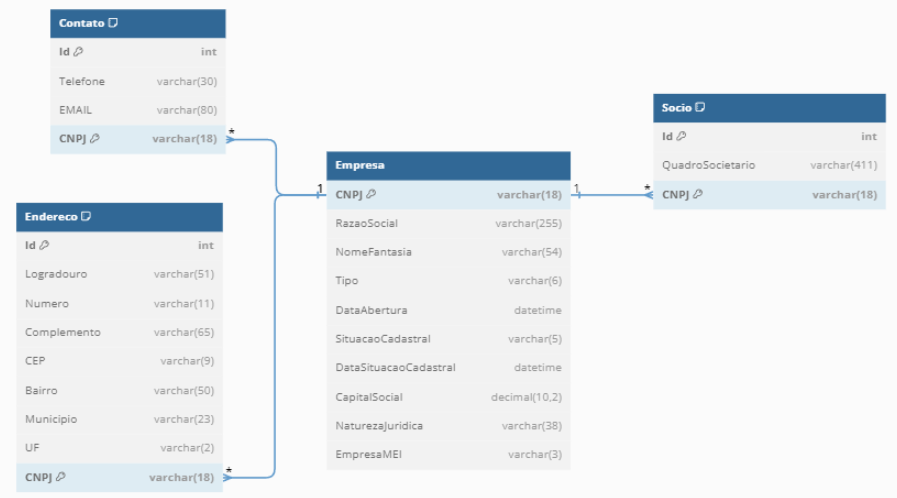
\includegraphics[width=\textwidth]{modelo_latex/figs/modelagem_dados.png}
    \caption{Modelagem de entidades e relacionamentos do banco de dados}
    \label{fig:diagrama_er}
\end{figure}

\subsubsection{Carga dos dados}

Com os dados modelados e o banco de dados criado, é necessário realizar a carga dos dados. Considerando que a carga dos dados só deve ser executada quando há dados para processar e que assim que a carga for realizada, sua função é finalizada, foi escolhido o serviço AWS Lambda. assim como na etapa de extração dos dados, o Lambda atende a necessidade da solução e apresenta o menor custo possível. A carga será realizada utilizando a linguagem Python e a biblioteca pymysql. Diferente da etapa de extração, o acionamento dessa tarefa é realizada por uma ação e não por agendamento periódico. Isso quer dizer que, sempre que os dados estiverem disponíveis, ele realizará a carga dos dados.

Visando uma melhor manutenção dos dados extraídos, foi sugerido um método de carga dos dados que permitia uma cópia dos dados inseridos no formato CSV. Dessa forma, caso houvesse algum problema com o banco de dados, a informação não seria perdida. Para isso, foi escolhido o serviço AWS S3. O S3 é um serviço de armazenamento de objetos que oferece escalabilidade, disponibilidade de dados, segurança e desempenho líderes do setor \cite{S3}. O S3 permite a criação de buckets, que são repositórios para armazenar arquivos e pastas. Com isso, é possível criar um bucket para armazenar os arquivos CSV gerados pelo processo de carga dos dados.

Com os dados disponibilizados no banco de dados, é necessário disponibilizar esses dados para os times de prospecção do cliente e análise de dados. Para isso, foi escolhido o serviço AWS RDS. Este serviço permite a criação de um banco de dados relacional, que pode ser acessado por qualquer ferramenta de análise de dados. Para esse projeto, foi escolhido o banco de dados Mysql, que é um banco de dados relacional de código aberto, com uma forte ênfase em extensibilidade e conformidade com padrões \cite{MySQL}. O Mysql amplamente utilizado no mercado, o que permite a fácil integração com ferramentas de análise de dados, como por exemplo o Power BI, que é a ferramenta utilizada pela empresa para a construção dos painéis de análise de dados.

Levando todas essas definições em consideração, a arquitetura proposta para a solução é apresentada na figura \ref{fig:arquitetura_proposta}.

\begin{figure}[H]
    \centering
    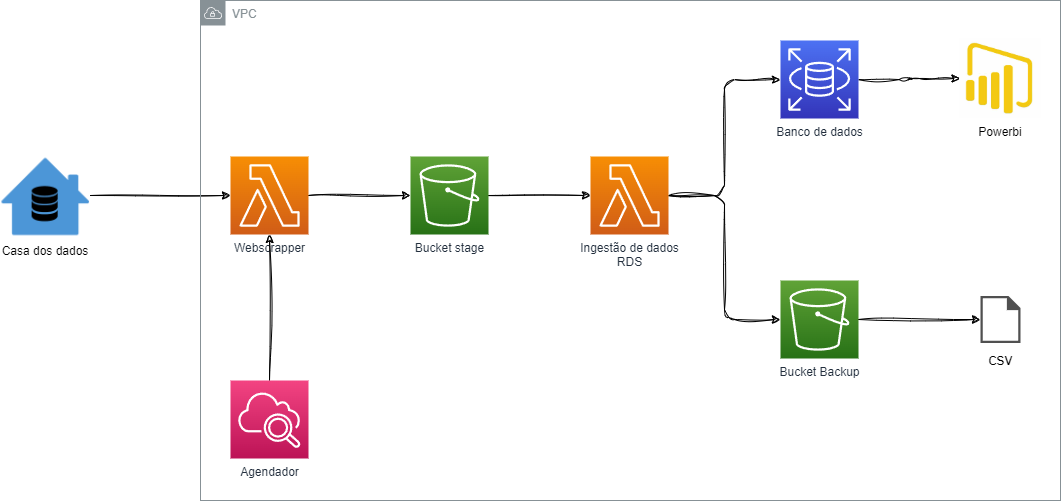
\includegraphics[width=\textwidth]{modelo_latex/figs/arquitetura_aws.png}
    \caption{Arquitetura proposta para a solução}
    \label{fig:arquitetura_aws}
\end{figure}